%\subsection{Problem}
%%%%%%%%%%%%%%%%%%%%%%%%%%%%%%%%%%%%%%%%%%%%%%%%%%%%%%%%%%%%%%%%%%%%%
\begin{frame}{Formation forming problem}
\begin{figure}
	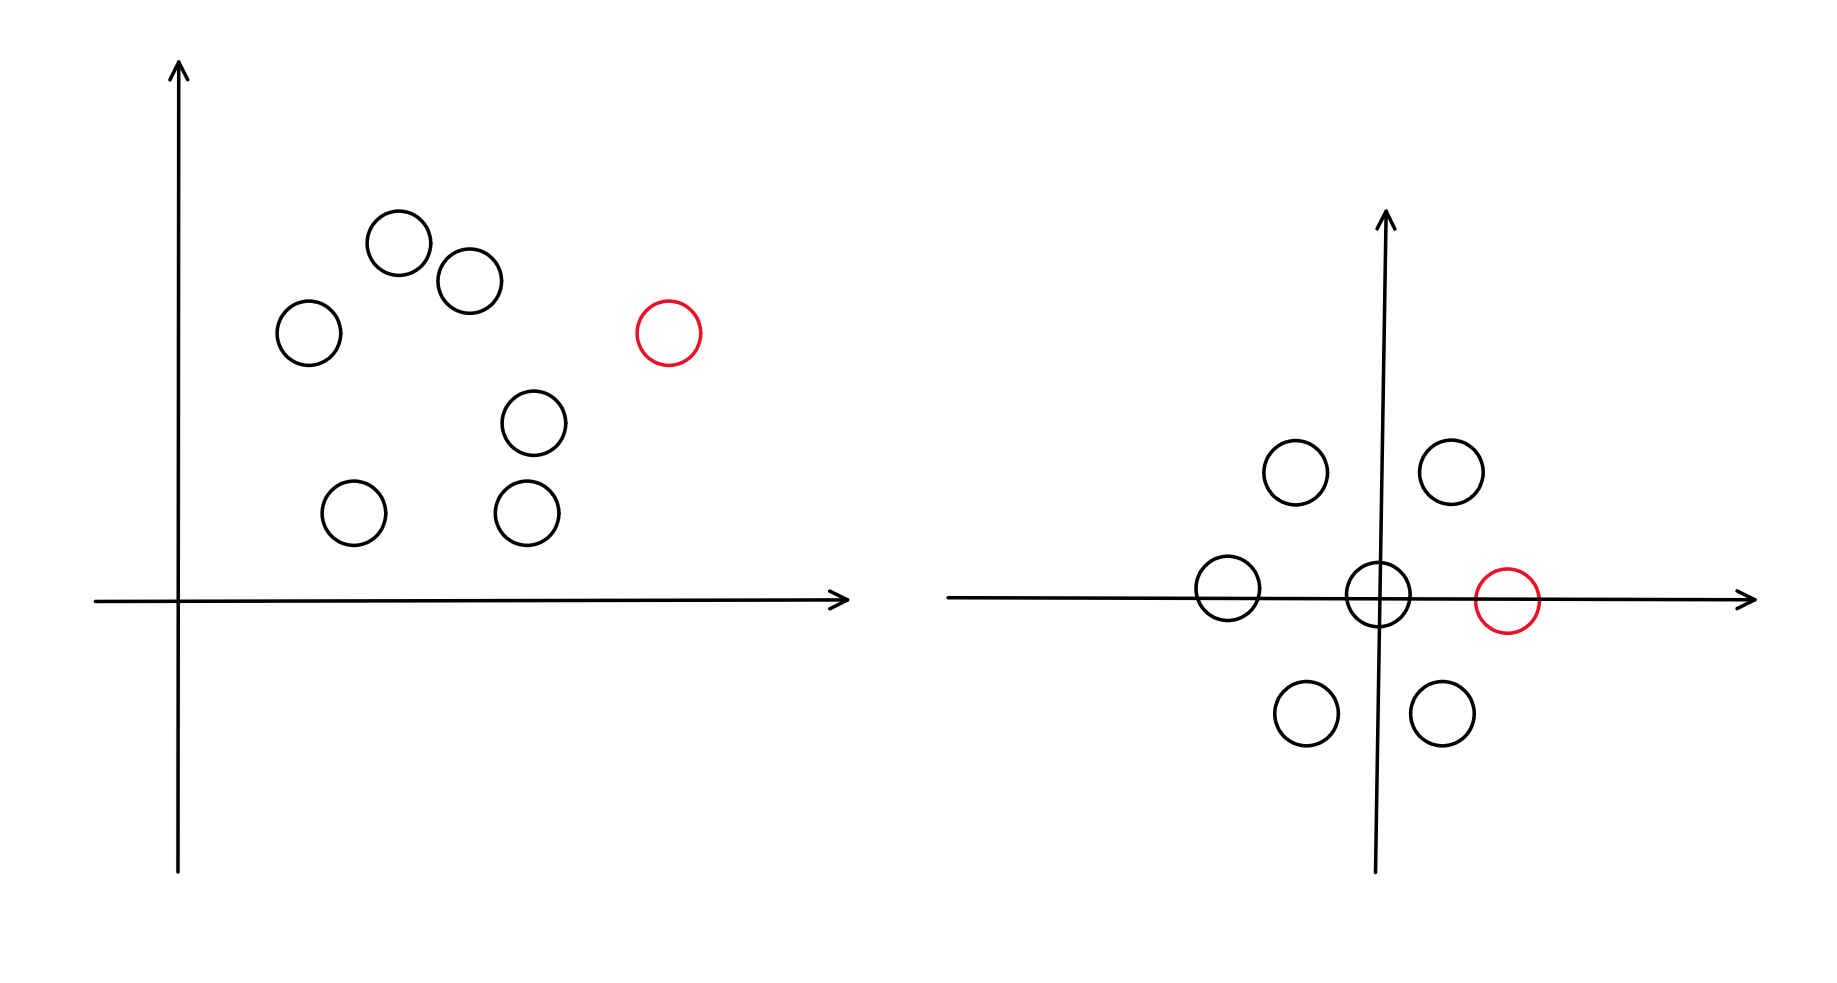
\includegraphics[width=0.55\textwidth]{figures/formation_control_schematic.png}
	%\caption{Oil Spills}
	%\label{fig:oilspills}
\end{figure}
\begin{itemize}
	\item A group of $N$ agents randomly deployed
	\item A single agent is externally "informed" (or controlled) to a desired location over time
	\item Each agent knows its $ID$ its desired offset from a commonly agreed location
	\item The dynamics of the complete system can be divided into
	\begin{itemize}
		\item Information flow dynamics over the network
		\item Local physical agent dynamics
	\end{itemize}	
\end{itemize}
\end{frame}
%%%%%%%%%%%%%%%%%%%%%%%%%%%%%%%%%%%%%%%%%%%%%%%%%%%%%%%%%%%%%%%%%%%%%
\begin{frame}{Core idea and key question}
	\begin{itemize}
		\item Vast literature on first order protocols (information flow dynamics)
		\item Real agents typically have higher order models
		\item \textbf{Core idea:} Wrap local tracking controller around simple information flow dynamics \footnote{Cortés, J. and Egerstedt, M., 2017. Coordinated control of multi-robot systems: A survey. SICE Journal of Control, Measurement, and System Integration, 10(6), pp.495-503.}
		\item \textbf{Core question:} Can we derive theoretical bounds on the loss in performance that depend on the local tracking performance?
	\end{itemize}
\end{frame}
%%%%%%%%%%%%%%%%%%%%%%%%%%%%%%%%%%%%%%%%%%%%%%%%%%%%%%%%%%%%%%%%%%%%%
\begin{frame}{Decoupled control Architecture}
	\begin{figure}[h!]
		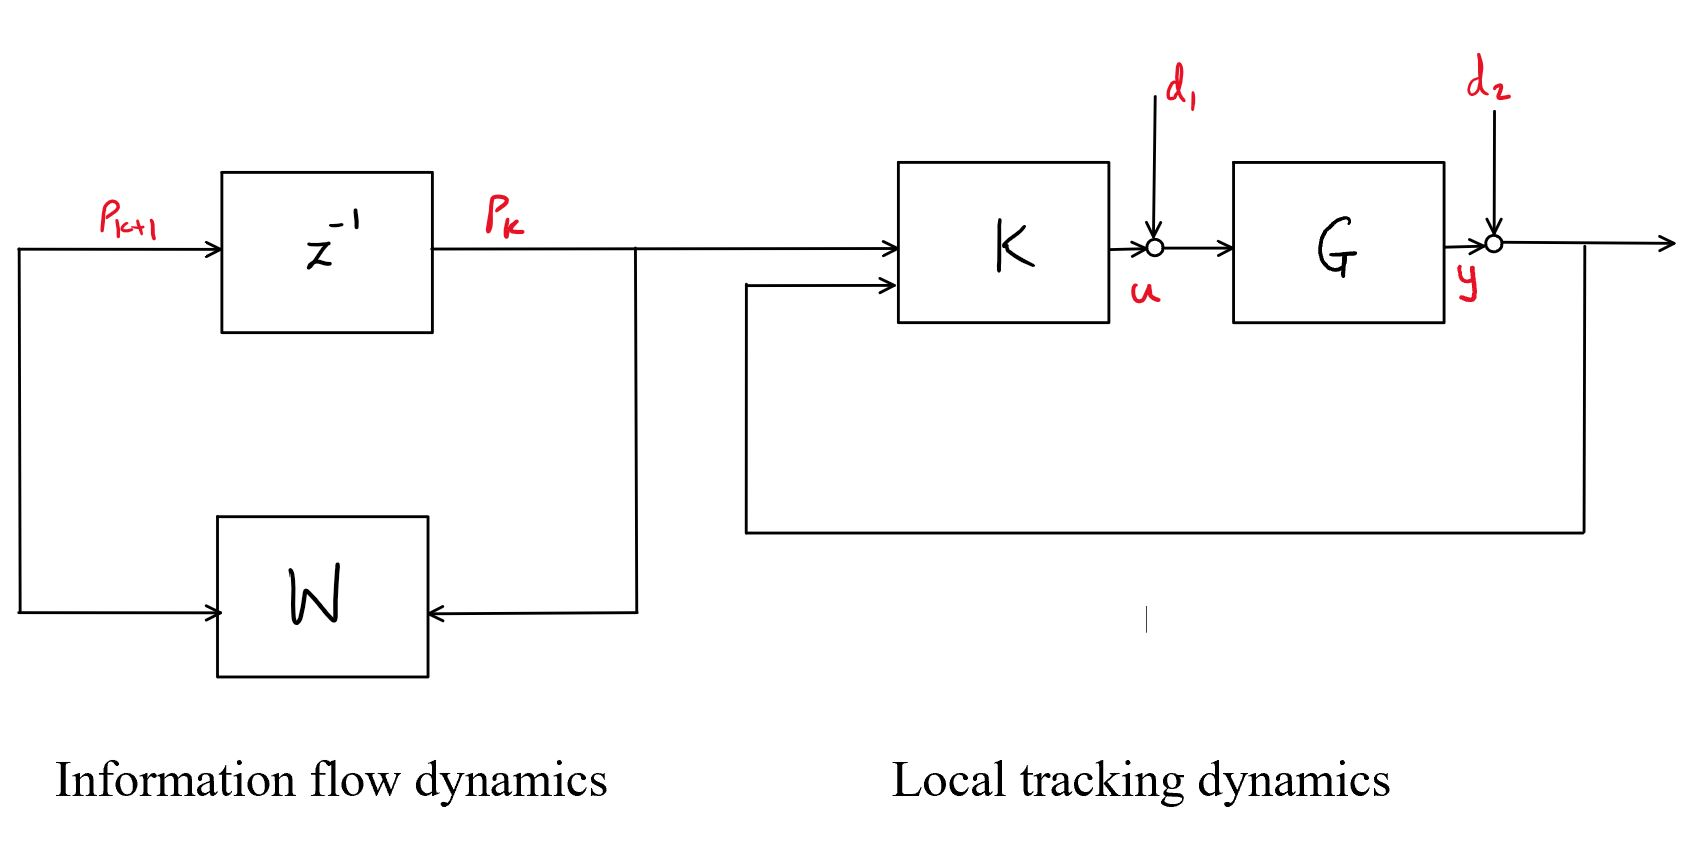
\includegraphics[width=10cm]{doc/2_Formation_control/decoupled_architecture.jpg}
		%\caption{}
		\label{fig:control_arch}	
	\end{figure}
Information flow dynamics
	\begin{equation*}\label{eqn:perturbed_information_flow_dynamics}
	\begin{split}
	p_{k+1}=W_cp_k \\
	\end{split}
	\end{equation*}
Physical agent dynamics (closed loop)	
	\begin{equation*}
	\begin{split}	
	\forall i \in \{1,\cdots, N\}:
	~~&\left\{
	\begin{array}{ll}
	x_i(k+1)&=Ax_i(k)+B_pp_i(k) + \bar{B}_dd_i(k) \\
	y_i(k) &=C1x_i(k) 
	\end{array}
	\right.
	\end{split}
	\end{equation*}
\end{frame}
%%%%%%%%%%%%%%%%%%%%%%%%%%%%%%%%%%%%%%%%%%%%%%%%%%%%%%%%%%%%%%%%%%%%%
\begin{frame}{Theory}
\begin{itemize}
	\item Scalable Analysis of information flow dynamics -> Positive systems theory\footnote{Rantzer, A., 2011, December. Distributed control of positive systems. In 2011 50th IEEE Conference on Decision and Control and European Control Conference (pp. 6608-6611). IEEE.}
	\item Local tracking loop Analysis -> generalized $H_2$ norm (induced $l_2$ to $l_{\infty}$ norm for non-linear systems)
	\item Scalable Analysis and Synthesis result
\end{itemize}
\end{frame}
%%%%%%%%%%%%%%%%%%%%%%%%%%%%%%%%%%%%%%%%%%%%%%%%%%%%%%%%%%%%%%%%%%%%%
\begin{frame}{Some simulation results}
	\begin{minipage}{0.45\textwidth}	
		\begin{figure}
			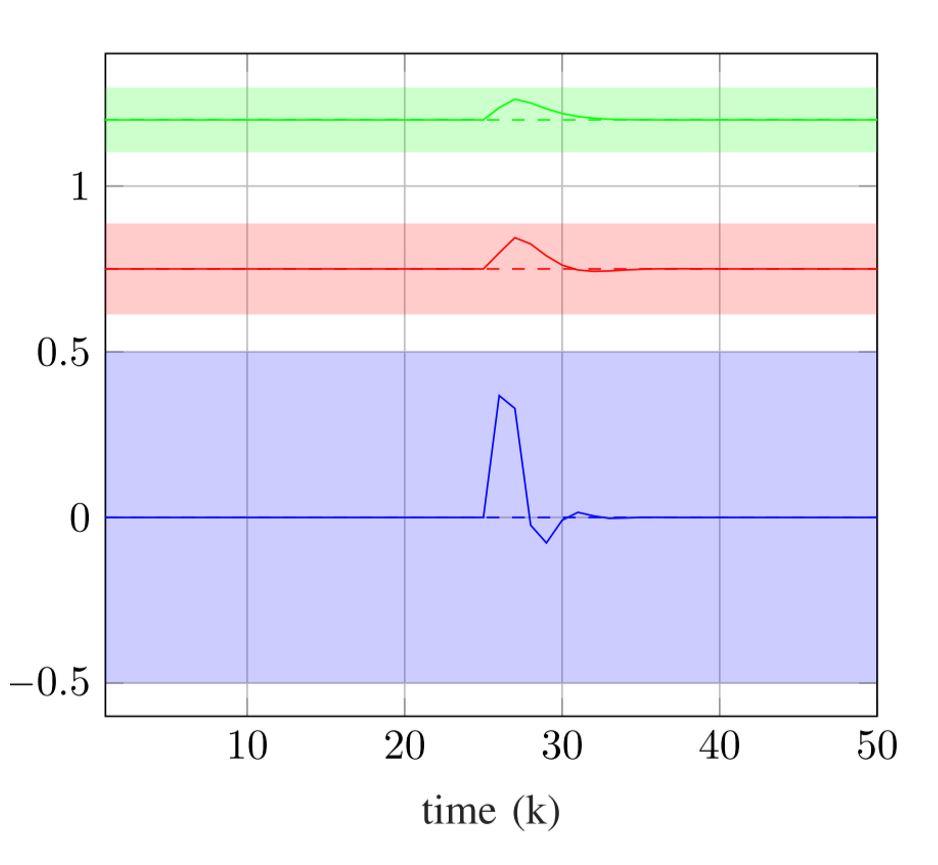
\includegraphics[width=1\textwidth]{doc/2_Formation_control/dist_rejection.jpg}
			%\caption{Fukushima Disaster (2011)}
			%\label{fig:fukushima_disaster}
		\end{figure}
		\begin{itemize}
			\item Disturbance rejection 
			\item Guaranteed peak bounds
		\end{itemize}		
	\end{minipage}
	\begin{minipage}{0.45\textwidth}	
		\begin{figure}
			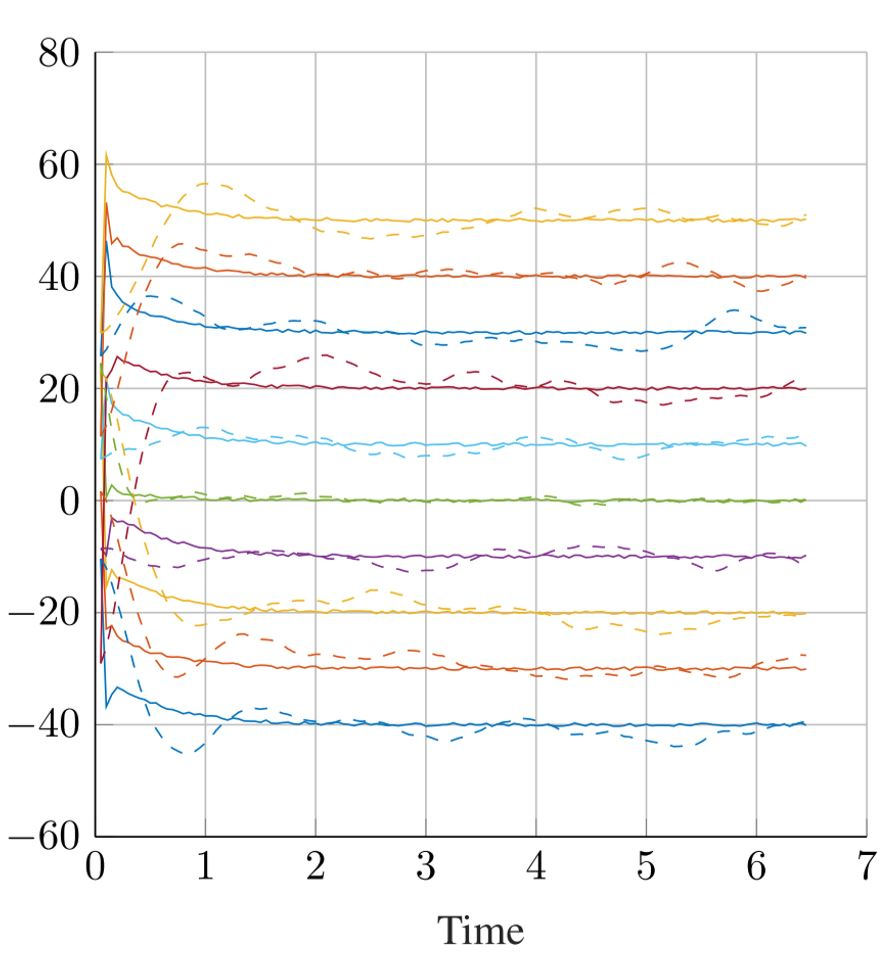
\includegraphics[width=1\textwidth]{doc/2_Formation_control/formation_stabilization.jpg}
			%\caption{Fukushima Disaster (2011)}
			%\label{fig:fukushima_disaster}
		\end{figure}
		\begin{itemize}
			\item Formation stabilization
		\end{itemize}		
	\end{minipage}	
\end{frame}	
%%%%%%%%%%%%%%%%%%%%%%%%%%%%%%%%%%%%%%%%%%%%%%%%%%%%%%%%%%%%%%%%%%%%%
\begin{frame}{Extensions to lossy networks}
	\begin{figure}[h!]
		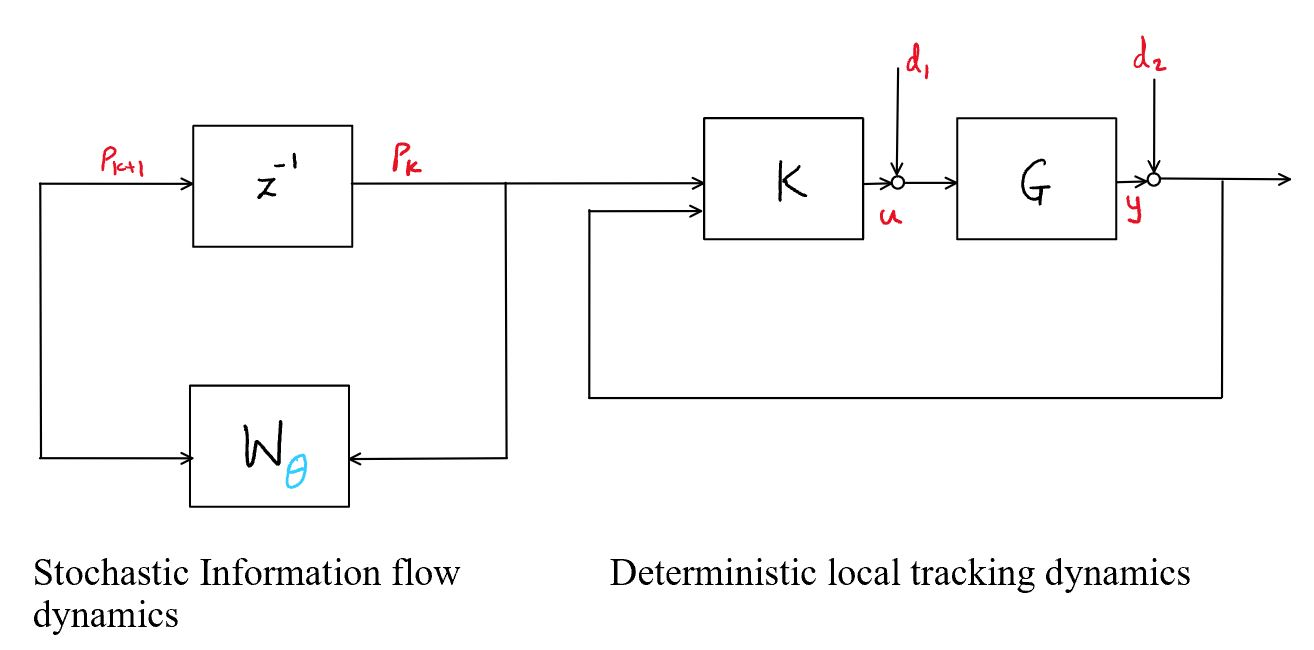
\includegraphics[width=9cm]{doc/2_Formation_control/stoch_decoupled_architecture.jpg}
		%\caption{}
		\label{fig:control_arch}	
	\end{figure}
	Stochastic information flow dynamics
	\begin{equation*}\label{eqn:perturbed_information_flow_dynamics}
	\begin{split}
	p_{k+1}=W_{\theta_k}p_k \\
	\end{split}
	\end{equation*}
	where $\{\theta_k\}_k$ is a finite Markov process 
	\begin{itemize}
		\item Want to derive LMIs to guarante performance e.g mean-square stability of the overall system
	\end{itemize}
\end{frame}
%%%%%%%%%%%%%%%%%%%%%%%%%%%%%%%%%%%%%%%%%%%%%%%%%%%%%%%%%%%%%%%%%%%%%
